\documentclass[aspectratio=169]{beamer}

% Simple student presentation for the Semester III evaluation.
% Compile on Overleaf with pdfLaTeX.
\usetheme{default}
\setbeamertemplate{navigation symbols}{}
\setbeamertemplate{footline}[frame number]
\usepackage{graphicx}
\graphicspath{{assets/}}
\usepackage{listings}
\usepackage{amsmath}
\usepackage{booktabs}

\title{Implementation of Distributed Graph Algorithms}
\subtitle{Social network problems using Apache Giraph}
\author{Kumar Shivam \and Archana Kumari}
\institute{School of Computer and Information Sciences\\University of Hyderabad}
\date{Semester III Evaluation\\11 December 2026}

\begin{document}

\begin{frame}
  \titlepage
\end{frame}

\begin{frame}{Problem definition}
\begin{itemize}
  \item We represent a social network as a graph.
  \item A vertex can be a person or a web page.
  \item An edge shows a connection between two vertices.
  \item A large graph has many vertices and edges, so one ordinary program can take a long time.
  \item We are studying how Apache Giraph can run these graph programs on Hadoop.
\end{itemize}
\end{frame}

\begin{frame}{Aim of the project}
\begin{itemize}
  \item Understand how Giraph processes one vertex at a time.
  \item Set up and use Hadoop, HDFS, YARN and Apache Giraph.
  \item Run basic graph programs and read their output.
  \item Implement Graph Burning and check it with a Python program.
  \item Keep our commands, code, input files and results in GitHub.
\end{itemize}
\end{frame}

\begin{frame}{Distributed technology used}
\begin{itemize}
  \item \textbf{Hadoop}: the platform on which our lab services run.
  \item \textbf{HDFS}: stores the graph files.
  \item \textbf{YARN}: starts and manages a submitted job.
  \item \textbf{Apache Giraph}: runs the graph algorithm.
  \item \textbf{Maven}: builds the Java code and creates the JAR file.
  \item \textbf{Git}: stores our code, reports and experiment records.
\end{itemize}
\end{frame}

\begin{frame}{Progress during the semester}
\begin{enumerate}
  \item We first learned Linux commands, graphs, Hadoop and distributed computing.
  \item We connected to the shared lab computer through SSH.
  \item We installed Java, Git, Maven and Hadoop services.
  \item We built Apache Giraph 1.4.0-SNAPSHOT with Maven.
  \item We tested HDFS and YARN with small graph files.
  \item We ran PageRank, in-degree, out-degree, BFS and shortest path.
  \item We added Graph Burning and checked its answer with Python.
  \item We tested the same workflow on a 348,087-vertex graph.
\end{enumerate}
\end{frame}

\begin{frame}{How Giraph runs our programs}
\begin{itemize}
  \item Yes, this is the model we used in our Giraph programs.
  \item Each vertex keeps its id, current value and neighbours.
  \item In one superstep, the vertex reads messages from neighbours.
  \item It updates its value and sends messages for the next superstep.
  \item Giraph repeats these supersteps until the program finishes.
\end{itemize}

\vspace{0.3cm}
\begin{block}{Simple idea}
  We write the rule for one vertex. Giraph applies the same rule to every vertex.
\end{block}
\end{frame}

\begin{frame}{Programs tested before Graph Burning}
\begin{tabular}{ll}
\toprule
Algorithm & What it calculates \\
\midrule
PageRank & Importance score based on incoming links \\
In-degree & Number of incoming edges \\
Out-degree & Number of outgoing edges \\
BFS & Minimum number of edges from a source \\
Shortest path & Minimum total edge weight from a source \\
\bottomrule
\end{tabular}

\vspace{0.4cm}
These programs helped us learn the input format, messages, supersteps, HDFS output and YARN execution.
\end{frame}

\begin{frame}{Graph Burning problem}
\begin{itemize}
  \item The input contains the graph and the source sequence.
  \item A source starts the fire in its assigned round.
  \item The fire spreads to connected vertices in later rounds.
  \item Every vertex records the first round in which it burns.
  \item We write \texttt{B round} for a burned vertex and \texttt{NB -1} if it is not burned.
\end{itemize}

\begin{block}{Example}
Source sequence: \texttt{3:8:6}. The sequence is an input schedule, not an optimized solution.
\end{block}
\end{frame}

\begin{frame}{Graph Burning workflow}
\begin{enumerate}
  \item We store the graph in plain-text adjacency-list files.
  \item We include the source round in each input record.
  \item Python checks the graph and calculates an expected answer.
  \item We upload the same input to HDFS.
  \item Giraph runs the Java program through YARN.
  \item We compare the Python and Giraph files.
\end{enumerate}
\end{frame}

\begin{frame}{Small example: one edge per round}
\begin{itemize}
  \item We use the nine-vertex path graph and the schedule \texttt{3:8:6}.
  \item Round 1 burns source 3 only.
  \item Round 2 spreads one edge from the old fire and ignites source 8.
  \item Round 3 repeats the same rule for source 6.
  \item A vertex first records the round in which it catches fire.
\end{itemize}
\vspace{0.15cm}
\begin{center}
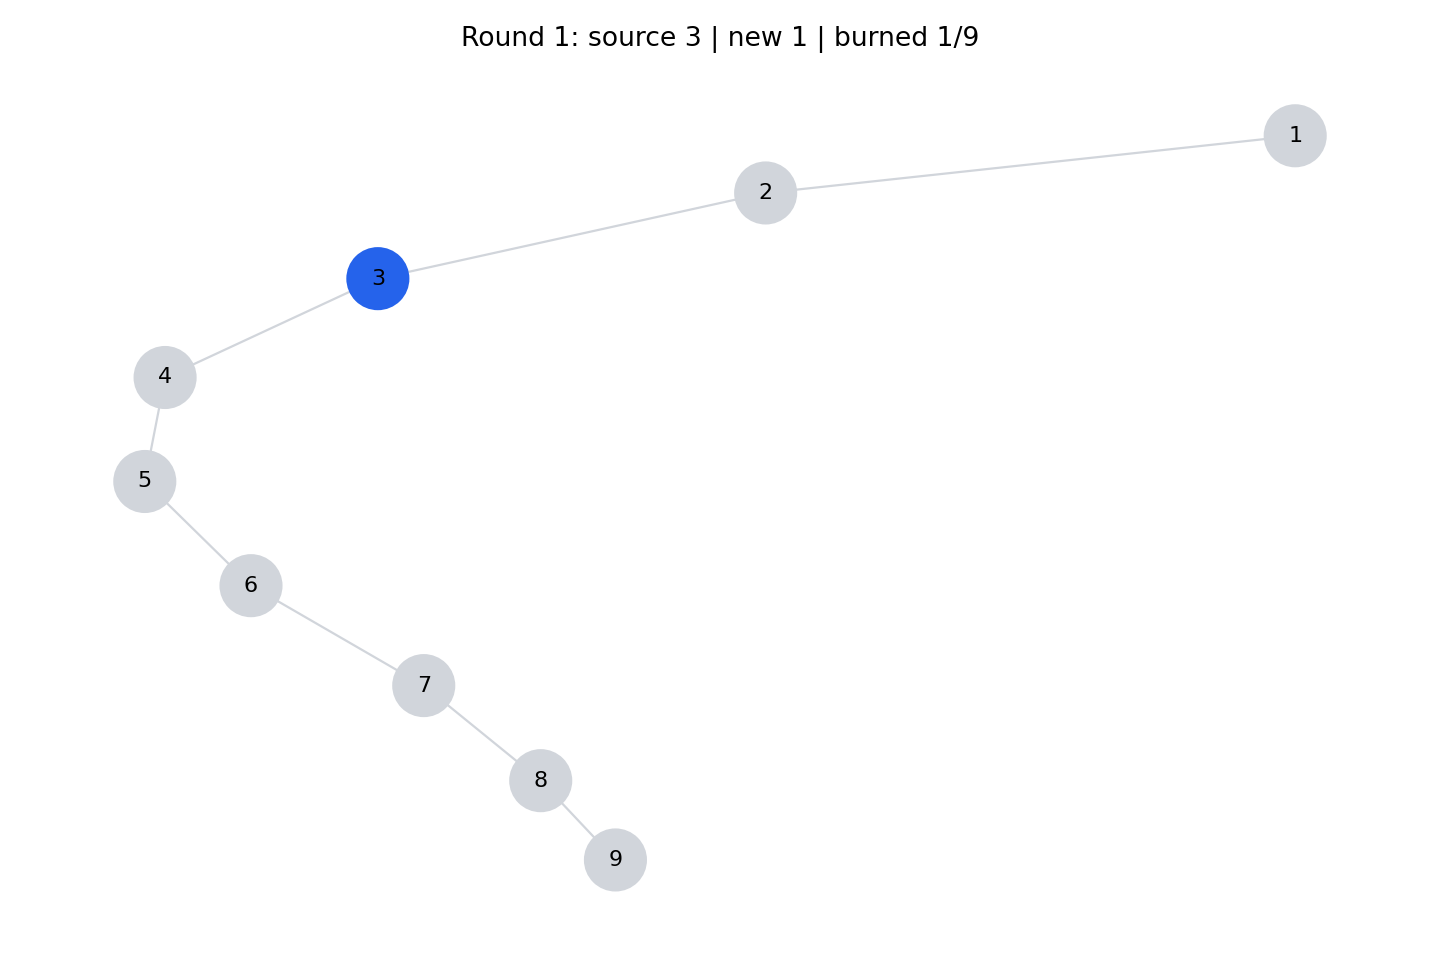
\includegraphics[width=.31\textwidth]{path9-round-01.png}\hspace{0.01\textwidth}
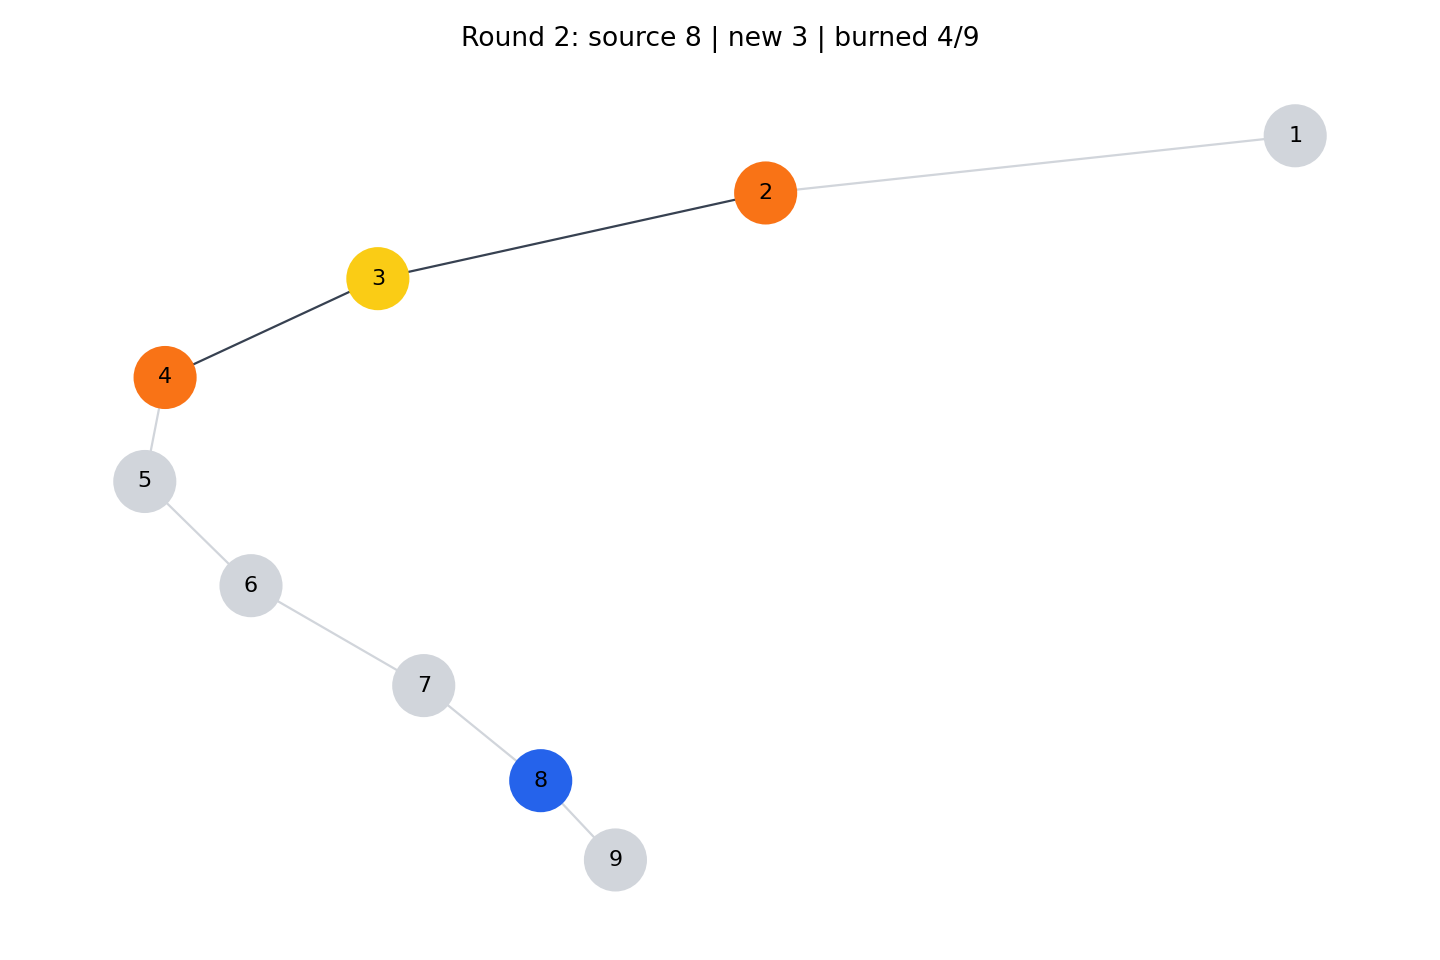
\includegraphics[width=.31\textwidth]{path9-round-02.png}\hspace{0.01\textwidth}
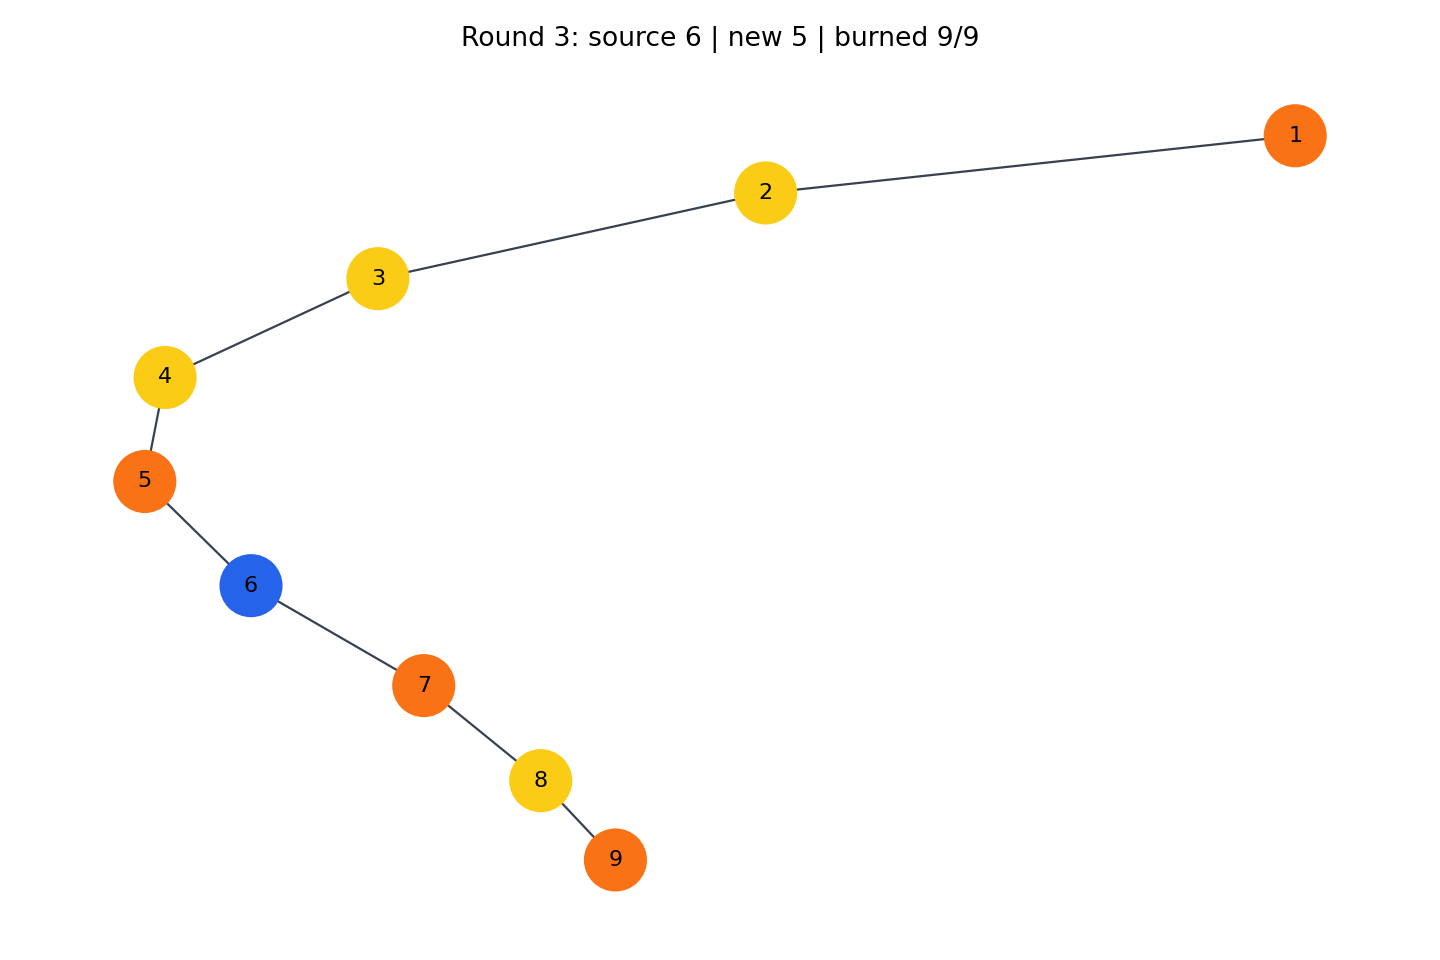
\includegraphics[width=.31\textwidth]{path9-round-03.png}
\end{center}
\scriptsize Round 1, Round 2 and Round 3. Burned vertices are highlighted in the saved NetworkX images.
\end{frame}

\begin{frame}[fragile]{Input formats used in the experiment}
\begin{columns}[T]
\column{.48\textwidth}
\textbf{Our scheduled plain-text format}
\begin{lstlisting}[basicstyle=\ttfamily\scriptsize]
3 1 2:1 4:1
8 2 7:1 9:1
6 3 5:1 7:1
\end{lstlisting}
The fields are vertex id, source round, then neighbour:weight pairs. A source round of 0 means that the vertex is not a source.

\column{.48\textwidth}
\textbf{Giraph adjacency-list format}
\begin{lstlisting}[basicstyle=\ttfamily\scriptsize]
1 0.0 2 1.0 3 1.0
2 0.0 1 1.0
3 0.0 1 1.0
\end{lstlisting}
This built-in format stores a vertex value followed by alternating neighbour ids and edge values. Our custom reader is needed for the source-round field.
\end{columns}
\end{frame}

\begin{frame}[fragile]{What the Java computation does}
\begin{lstlisting}[language=Java,basicstyle=\ttfamily\tiny,aboveskip=2pt,belowskip=2pt]
long currentRound = getSuperstep() + 1;
double storedValue = vertex.getValue().get();
if (storedValue <= 0) {
  double firstArrival = Double.MAX_VALUE;
  for (DoubleWritable message : messages)
    firstArrival = Math.min(firstArrival, message.get());
  if (storedValue == -currentRound)
    firstArrival = Math.min(firstArrival, currentRound);
  if (firstArrival != Double.MAX_VALUE) {
    vertex.getValue().set(firstArrival);
    for (Edge<LongWritable, FloatWritable> edge : vertex.getEdges())
      sendMessage(edge.getTargetVertexId(),
                  new DoubleWritable(currentRound + 1));
  }
}
\end{lstlisting}
\begin{itemize}
  \item The negative input value keeps a scheduled source until its round.
  \item A positive value is the first burn round.
  \item Messages move the fire one edge per superstep.
\end{itemize}
\end{frame}

\begin{frame}[fragile]{Python check before the Giraph job}
\begin{lstlisting}[language=bash,basicstyle=\ttfamily\scriptsize]
python3 show_burning_rounds.py scheduled-input \\
  --output-dir preview
hdfs dfs -cat giraph-output/part-00000 > giraph-actual.tsv
diff -u preview/expected.tsv giraph-actual.tsv
\end{lstlisting}
\begin{itemize}
  \item \texttt{show\_burning\_rounds.py} applies the same one-edge-per-round rule.
  \item It saves the expected table and a PNG for each round.
  \item Exit code 0 from \texttt{diff} means the Python and Giraph rows match exactly.
\end{itemize}
\end{frame}

\begin{frame}{Larger example: 30 vertices}
\begin{columns}[T]
\column{.52\textwidth}
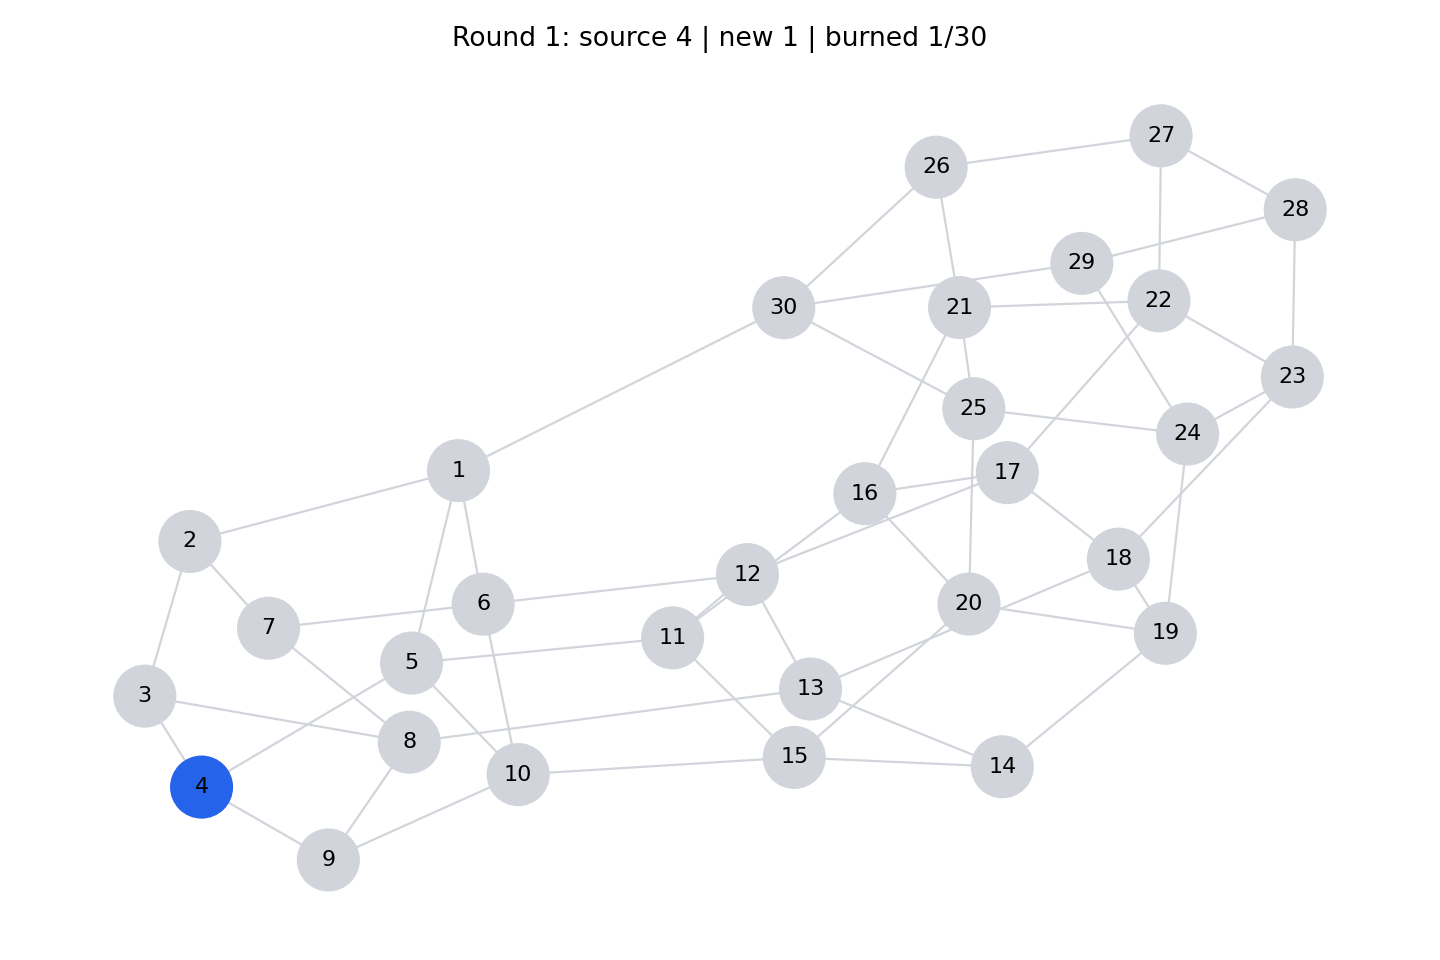
\includegraphics[width=\textwidth]{graph30-round-01.png}
\column{.44\textwidth}
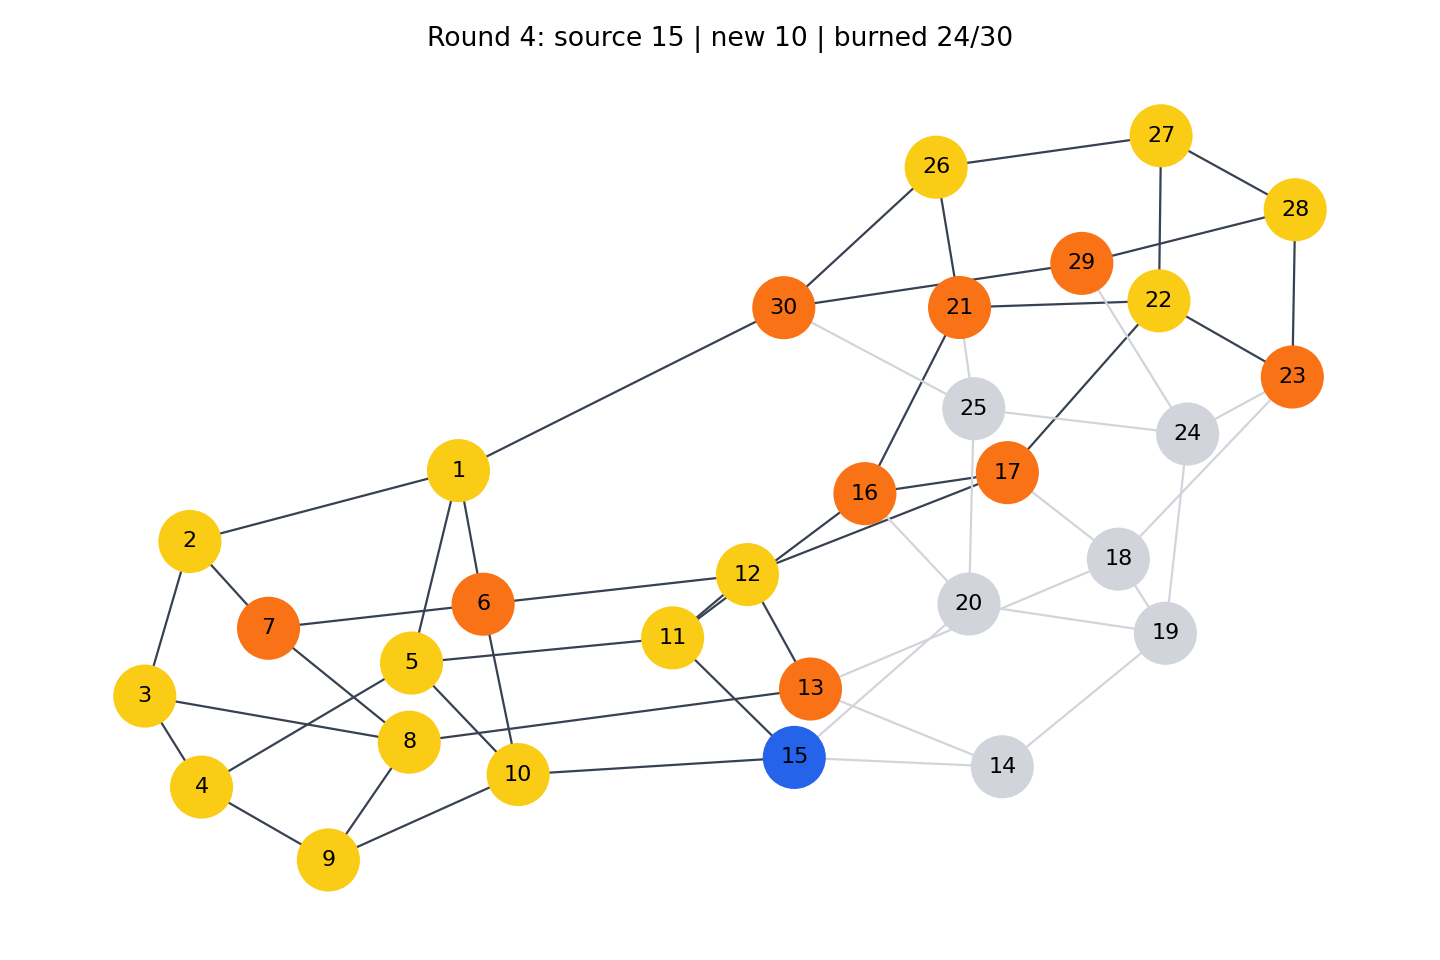
\includegraphics[width=\textwidth]{graph30-round-04.png}
\end{columns}
\vspace{0.15cm}
The same input-driven program was run on a 30-vertex graph. These are saved experiment images, not a hand-drawn illustration. The colours show which vertices have burned by each round.
\end{frame}

\begin{frame}{Input and output format}
\textbf{Input example:}\\[-2pt]
\texttt{3 1 2:1 4:1}\\
\texttt{8 2 7:1 9:1}\\
\texttt{6 3 5:1 7:1}

The first value is the vertex id. The second value is its source round. The remaining values are neighbour and weight pairs.

\textbf{Output example:}\\[-2pt]
\texttt{3  B  1}\\
\texttt{8  B  2}\\
\texttt{9  NB -1}
\end{frame}

\begin{frame}{Python verification and Giraph execution}
\begin{itemize}
  \item Python calculates the answer independently.
  \item Giraph reads the HDFS input and runs the Java computation.
  \item Both outputs contain the vertex id, burn status and first burn round.
  \item We compare the two files line by line.
  \item Exit code 0 means the two tested files matched exactly.
\end{itemize}

\begin{block}{Why this is useful}
Python gives us an expected answer before we check the Giraph result.
\end{block}
\end{frame}

\begin{frame}{Large graph experiment}
\begin{tabular}{lr}
\toprule
Measure & Result \\
\midrule
Vertices & 348,087 \\
Undirected connections & 1,128,693 \\
Scheduled source rounds & 8 \\
Burned vertices & 243,095 \\
Unburned vertices & 104,992 \\
Python and Giraph rows & 348,087 each \\
\bottomrule
\end{tabular}

\vspace{0.4cm}
This was a reproducible random schedule. We did not claim that it was optimal.
\end{frame}

\begin{frame}{Verification and runtime: large graph}
\scriptsize
\begin{columns}[T]
\column{.48\textwidth}
\begin{block}{Correctness check}
\begin{tabular}{lr}
Python expected rows & 348,087 \\
Giraph actual rows & 348,087 \\
Comparison & \textbf{exit code 0} \\
Burned / unburned & 243,095 / 104,992
\end{tabular}
\end{block}

\column{.48\textwidth}
\begin{alertblock}{Measured timing}
\begin{tabular}{ll}
Python preview & about 20 minutes \\
Giraph run & \textbf{54.887 seconds}
\end{tabular}
\end{alertblock}
\end{columns}

\vspace{0.25cm}
\small Python wrote every round's node table and edge list. Giraph computed and wrote only the final result, so these timings measure different amounts of work.
\end{frame}

\begin{frame}{Results and discussion}
\begin{itemize}
  \item The basic programs ran successfully on small graphs.
  \item Graph Burning ran on small, medium and large inputs.
  \item The 348,087-vertex Giraph output matched the Python output.
  \item The Giraph run took about 54.887 seconds after YARN was ready.
  \item The Python preview took longer because it saved every round's state and edges.
\end{itemize}
\end{frame}

\begin{frame}{Our work this semester}
\begin{itemize}
  \item We prepared the shared SSH lab environment.
  \item We built and tested the Apache Giraph JAR.
  \item We tried JSON and then used plain-text graph input.
  \item We wrote a runner so that we could repeat a Giraph experiment.
  \item We implemented Graph Burning input parsing and computation.
  \item We added Python checking, prediction and comparison scripts.
  \item We kept weekly reports, study notes, datasets and results in GitHub.
\end{itemize}
\end{frame}

\begin{frame}{Conclusion and future work}
\begin{itemize}
  \item We now have a working Hadoop, YARN and Giraph setup.
  \item We ran several Giraph graph algorithms and learned how their output is produced.
  \item We implemented and checked the current Graph Burning workflow.
  \item Next we will finalise the burning rule, constraints and evaluation measures with our guide.
  \item We will test larger graphs and study parallel execution by varying workers and containers.
  \item We will optimise the source sequence, compare simple methods with existing research, and prepare a paper from the results.
\end{itemize}
\end{frame}

\begin{frame}{References}
\begin{itemize}
  \item Apache Giraph: \url{https://giraph.apache.org/}
  \item Apache Hadoop: \url{https://hadoop.apache.org/}
  \item Stanford SNAP datasets: \url{https://snap.stanford.edu/data/}
  \item Project repository: \url{https://github.com/25mcmc34-kumarshivam/APACHE-GIRAPH-PROJECT-}
\end{itemize}
\end{frame}

\end{document}
